\chapter{Volladdierer}

\section{Einführung}

Ein Volladdierer ist eine Schaltung, die zwei Dualzahlen zusammenzählt. Dabei beginnt er bei der letzten Stelle, genau so, wie eine Addition „von Hand“ ausgeführt wird. Hier ein kleines Beispiel:\index{Volladdierer}\index{Addition}

Die Dualzahlen a\textsubscript{3}a\textsubscript{2}a\textsubscript{1}a\textsubscript{0} und b\textsubscript{3}b\textsubscript{2}b\textsubscript{1}b\textsubscript{0} sollen addiert werden.

\begin{table}[htbp]
  \centering
  \begin{tabular}{ccccc}
    \toprule
     & a\textsubscript{3} & a\textsubscript{2} & a\textsubscript{1} & a\textsubscript{0} \\
    \midrule
    + & b\textsubscript{3} & b\textsubscript{2} & b\textsubscript{1} & b\textsubscript{0} \\
     & Ü\textsubscript{3} & Ü\textsubscript{2} & Ü\textsubscript{1} &  \\
    Ü\textsubscript{4} & S\textsubscript{3} & S\textsubscript{2} & S\textsubscript{1} & S\textsubscript{0} \\
    \bottomrule
  \end{tabular}
\end{table}

Die Dualzahlen werden untereinander geschrieben. Danach wird die Summe aus a\textsubscript{0} + b\textsubscript{0} gebildet und der Übertrag Ü\textsubscript{1} unter a\textsubscript{1} und b\textsubscript{1} geschrieben. So läuft die Addition weiter bis zum Übertrag Ü\textsubscript{4}, der vor die Summen S\textsubscript{3} S\textsubscript{2} S\textsubscript{1} S\textsubscript{0} gesetzt wird.\index{Addition}

Dabei kann der Volladdierer (VA) nur zwei einstellige Dualzahlen addieren, wodurch ein kleiner Kunstgriff nötig wird um größere Dualzahlen zu addieren. Doch dazu später mehr.\index{Volladdierer}

Zuerst stellt sich die Frage: Wie werden Dualzahlen eigentlich addiert? Dabei gelten natürlich genau wie bei der Addition im Dezimalsystem auch bestimmte Regeln. Diese sind in der Logik-Tafel abgebildet. Dabei stellt A eine zu addierende Variable dar, B die andere. Diese beiden Werte A und B werden also zu der Summe S und dem Übertrag Ü zusammengefasst.\index{Addition}\index{Dezimalsystem}

\begin{table}[htbp]
  \centering
  \begin{tabular}{cccc}
    \toprule
    A & B & S & Ü \\
    \midrule
    0 & 0 & 0 & 0 \\
    0 & 1 & 1 & 0 \\
    1 & 0 & 1 & 0 \\
    1 & 1 & 0 & 1 \\
    \bottomrule
  \end{tabular}
\end{table}

Ein Volladdierer besteht eigentlich aus zwei Halbaddierern, die zwei einstellige Dualzahlen addieren können, jedoch ohne Übertrag. Durch die Zusammenschaltung dieser beiden Halbaddierer ist es möglich, eine Summe samt Übertrag zu bilden. Da die Volladdierer aber als fertige ICs angeboten werden, empfiehlt es sich, diese zu verwenden.\index{Volladdierer}\index{Halbaddierer}

Doch nun zu dem vorher angesprochenen Problem. Wie sieht eine Volladdierer-Schaltung aus, mit der man zwei vierstellige Dualzahlen summieren kann?\index{Volladdierer}

Bei diesem Problem hilft uns wiederum das Schieberegister. Wenn man die Register mit den schon gespeicherten Daten an einen VA in der angegebenen Weise anschliesst, so stehen pro Taktimpuls immer nur zwei Werte der beiden Dualzahlen zur Addition zur Verfügung. Es beginnt mit den beiden Werten a\textsubscript{0} und b\textsubscript{0}. Diese werden nun in den VA eingegeben, der sie addiert. Am Ausgang S steht dann die Summe dieser beiden Zahlen und am Ausgang Ü der Übertrag. Bei einem erneuten Taktimpuls gelangen nun die beiden Dualwerte a\textsubscript{1} und b\textsubscript{1}, die ja nach dem letzten Taktimpuls den Platz von a\textsubscript{0} und b\textsubscript{0} eingenommen haben, an den VA.\index{Taktimpuls}\index{Addition}

Das JK-Flipflop unterhalb der Schieberegister, das vor diesem Taktimpuls den Wert Ü\textsubscript{1} am Eingang hatte, hat nun den Wert Ü\textsubscript{1} am Ausgang Q. Dieser Ausgang Q ist nun mit einem weiteren Eingang C des VA verbunden. Es liegen also an den Eingängen des Volladdierers die Werte a\textsubscript{1} (an A), b\textsubscript{1} (an B) und Ü\textsubscript{1} an C. Diese werden wiederum addiert und erscheinen als Summe S und als Übertrag Ü an dessen Ausgängen.\index{JK-Flipflop}\index{Taktimpuls}

Zuvor wurde jedoch der Ausgang S des VA mit dem J-Eingang des Serienaddierers verbunden. Nachdem nun die Summe a\textsubscript{0} + b\textsubscript{0} gebildet wurde und ein erneuter Taktimpuls die Werte a\textsubscript{3}, a\textsubscript{2} und a\textsubscript{1} um eine Stelle weiter nach rechts geschoben hat (ebenso die Werte b\textsubscript{3}, b\textsubscript{2} und b\textsubscript{1}), sind in den Schieberegistern folgende Werte gespeichert.\index{Taktimpuls}

\begin{quote}
  Register A: X,  a\textsubscript{3}, a\textsubscript{2}, a\textsubscript{1}
\end{quote}


\begin{quote}
  Register B: S\textsubscript{0}, b\textsubscript{3}, b\textsubscript{2}, b\textsubscript{1}
\end{quote}


In dem JK-Flipflop befindet sich der Übertrag Ü\textsubscript{1}.\index{JK-Flipflop}

Nun tritt die erneute Addition der Variablen an A, B und C des VA auf. Es wird also die Summe a\textsubscript{1} + b\textsubscript{1} + Ü\textsubscript{1} gebildet. Dabei wird die Summe S\textsubscript{1} gebildet, die wiederum am J-Eingang des unteren Schieberegisters anliegt und bei einem erneuten Taktimpuls als Information aufgenommen wird. Der Übertrag Ü\textsubscript{2}, der bei der Addition entsteht und an den J-Eingang des Flipflops gelegt wird, wird auch von diesem beim nächsten Impuls aufgenommen und erscheint dann am Ausgang Q um von dort bei einer erneuten Addition übernommen zu werden.\index{Addition}\index{Taktimpuls}

Es befinden sich also jetzt folgende Werte in den Registern:

\begin{quote}
  Register A: X,   X, a\textsubscript{3}, a\textsubscript{2}
\end{quote}


\begin{quote}
  Register B: S\textsubscript{1}, S\textsubscript{0}, b\textsubscript{3}, b\textsubscript{2}
\end{quote}


In dem JK-Flipflop befindet sich der Übertrag Ü\textsubscript{2}.\index{JK-Flipflop}

Bei einem erneuten Taktimpuls wird die Summe der Werte a\textsubscript{2}, b\textsubscript{2} und Ü\textsubscript{2} gebildet. Es erscheint dann am Ausgang S des VA die gebildete Summe S\textsubscript{2} und der Übertrag Ü\textsubscript{3}.\index{Taktimpuls}

Diese Art der Addition wird so weit fortgesetzt bis sämtliche Variablen addiert sind. Nachdem die letzte Summierung geschehen ist und die letzte Summe in dem unteren Schieberegister abgespeichert wurde, sind die Werte wie folgt in den Registern:\index{Addition}

Register A: X,   X,  X,  X

Register B: S\textsubscript{3}, S\textsubscript{2}, S\textsubscript{1}, S\textsubscript{0}

In dem JK-Flipflop befindet sich der Übertrag Ü\textsubscript{4}.\index{JK-Flipflop}

Der Übertrag Ü\textsubscript{4} kann nun aus dem JK-Flipflop entnommen werden und vor die Summe S\textsubscript{3}, S\textsubscript{2}, S\textsubscript{1}, S\textsubscript{0} gesetzt werden. Der Sachverhalt der Verschiebung innerhalb des Registers und die Addition der einzelnen Variablen zu einer Summe S und dem Übertrag Ü ist in der folgenden Tabelle noch einmal zusammengefasst.\index{JK-Flipflop}\index{Addition}

Schieberegister A:

\begin{table}[htbp]
  \centering
  \begin{tabular}{ccccc}
    \toprule
    t & Stelle 3 & Stelle 2 & Stelle 1 & Stelle 0 \\
    \midrule
    0 & a\textsubscript{3} & a\textsubscript{2} & a\textsubscript{1} & a\textsubscript{0} \\
    1 & X & a\textsubscript{3} & a\textsubscript{2} & a\textsubscript{1} \\
    2 & X & X & a\textsubscript{3} & a\textsubscript{2} \\
    3 & X & X & X & a\textsubscript{3} \\
    4 & X & X & X & X \\
    \bottomrule
  \end{tabular}
\end{table}

Schieberegister B:

\begin{table}[htbp]
  \centering
  \begin{tabular}{ccccc}
    \toprule
    t & Stelle 3 & Stelle 2 & Stelle 1 & Stelle 0 \\
    \midrule
    0 & b\textsubscript{3} & b\textsubscript{2} & b\textsubscript{1} & b\textsubscript{0} \\
    1 & S\textsubscript{0} & b\textsubscript{3} & b\textsubscript{2} & b\textsubscript{1} \\
    2 & S\textsubscript{1} & S\textsubscript{0} & b\textsubscript{3} & b\textsubscript{2} \\
    3 & S\textsubscript{2} & S\textsubscript{1} & S\textsubscript{0} & b\textsubscript{3} \\
    4 & S\textsubscript{3} & S\textsubscript{2} & S\textsubscript{1} & S\textsubscript{0} \\
    \bottomrule
  \end{tabular}
\end{table}

JK-Flipflop:\index{JK-Flipflop}

\begin{table}[htbp]
  \centering
  \begin{tabular}{cc}
    \toprule
    t & Q \\
    \midrule
    0 & X \\
    1 & Ü\textsubscript{1} \\
    2 & Ü\textsubscript{2} \\
    3 & Ü\textsubscript{3} \\
    4 & Ü\textsubscript{4} \\
    \bottomrule
  \end{tabular}
\end{table}

\begin{figure}[htbp]
  \centering
  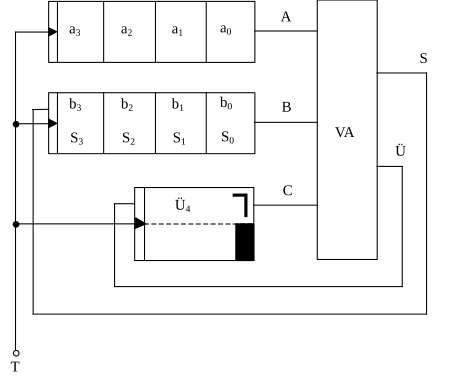
\includegraphics[width=.8\linewidth]{media/abb-72}
  \caption{Schaltbild Serienaddierer}
\end{figure}

Das obere Schieberegister A, das untere B, das JK-Flipflop und der Volladdierer bilden zusammen eine Einheit. Da diese Schaltung mehrere Variablen, also eine „Serie von Bits“, addieren kann, nennt man diese Schaltung auch einen Serienaddierer.\index{JK-Flipflop}\index{Volladdierer}

Der Takt T, der an den beiden Schieberegistern und dem Flipflop liegt muss an den Eingang T angelegt werden. Weiterhin müssen die dualen Zahlen a\textsubscript{3}a\textsubscript{2}a\textsubscript{1}a\textsubscript{0} und b\textsubscript{3}b\textsubscript{2}b\textsubscript{1}b\textsubscript{0} über die Setz- und Rücksetzeingänge in die Register geladen werden. Diese Eingänge sind hier der Übersicht wegen nicht eingezeichnet.

Wenn die Schaltung aufgebaut und in Betrieb genommen wird, empfiehlt es sich zuerst Einzelimpulse an den Takteingang T zu legen. So kann die Schaltung Schritt für Schritt beobachtet  und kontrolliert werden. Danach ist ein Betrieb mit höherer Taktfrequenz möglich.\index{Takteingang}\index{Taktfrequenz}

